\newif\ifvimbug
\vimbugfalse

\ifvimbug
\begin{document}
\fi

\exercise{Linear Classification}

In this exercise, you will use the dataset \texttt{ldaData.txt}, containing 137 feature points $\vec x$. The first 50 points belong to class $C_1$, the second 43 to class $C_2$, the last 44 to class $C_3$.


\begin{questions}
%----------------------------------------------

\begin{question}{Discriminative and Generative Models}{4}
Explain the difference between discriminative and generative models and give an example for each case.
Which model category is generally easier to learn and why?
 
\begin{answer}
\textbf{Generative models} first use the underlying data to deduce properties of the underlying probability distribution in form of the class-doncitional densties $p(x|C_k)$ for each class $C_k$. Seperatly they infer the prior class probabilities $p(C_k)$. After that, they use Bayes'theorem  in the form 
\begin{equation}
	\frac{p(x|C_k) p(C_k)}{p(x)}
\end{equation}
to fint the posteriori class probabilities $p(C_k|x)$. Now decision theory is used to determine class membership. 

Since in theory we can use these distribution to create new data, this is called a gernative model. Also note that generative models also work when modeling the joint distribution $p(x, C_k)$ and normalizing. 


\textbf{Discriminative models} determine the posterior class probabilities $p(C_k|x)$ directly. After that decision theory is used to each new input to a class. 


Because generative models need the joint distribution $p(x,C_k)$ for calculating the posterior distribution, instead of deriving it directly, they're much harder to train. This is especially true if $x$ is highly dimensional, since then we need a very big dataset to model class-doncitional densities correctly.

 

\end{answer}

\end{question}

%----------------------------------------------

\begin{question}{Linear Discriminant Analysis}{12}
Use Linear Discriminant Analysis to classify the points in the dataset, i.e., assume Gaussian distributions in each class with equal covariances and use the posterior distributions for assigning classes. Attach two plots with the data points using a different color for each class: one plot with the original dataset, one with the samples classified according to your LDA classifier. Attach a snippet of your code and discuss the results. How many samples are misclassified? (You are allowed to use built-in functions for computing the mean and the covariance.)

\begin{answer}\end{answer}
First, lets have a look at the data \ref{fig:classData}:
\begin{figure}[H]
	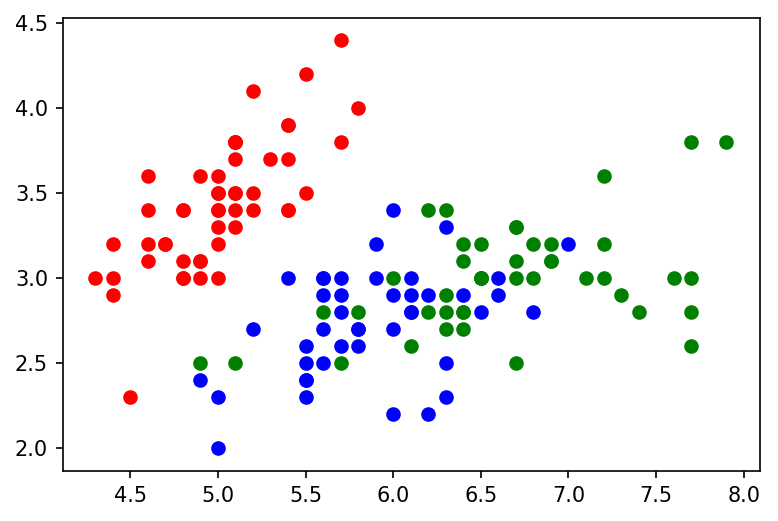
\includegraphics[width=0.6\linewidth]{pictures/OriginalData.png}
	\centering
	\caption{The given data. Three classes of points, represent by the colors: [red, blue, green].}
	\label{fig:classData}
\end{figure}

For our classifier we chosed a Maximum Likelihood model with a Gaussian Prior.
The classifier yields following result \ref{classifier}
\begin{figure}[H]
	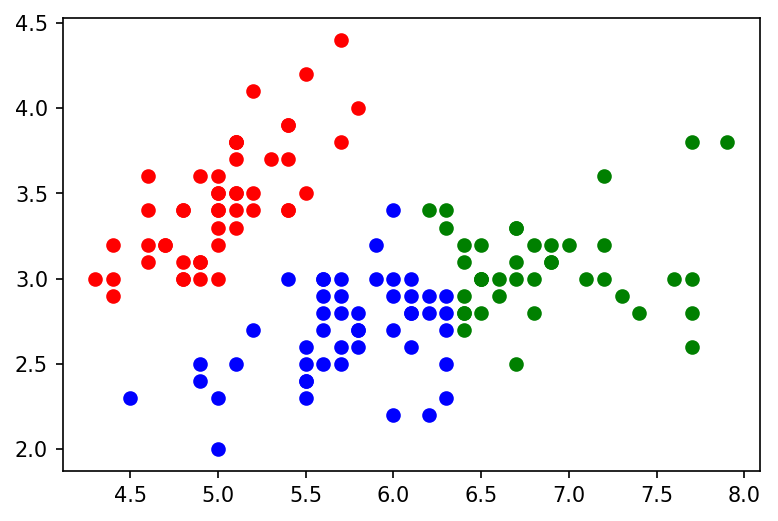
\includegraphics[width=0.6\linewidth]{pictures/OurClassifier.png}
	\centering
	\caption{The classified data by our Maximum likelihood. 19 Points are missclassified.}
	\label{fig:classifier}
\end{figure}

Since there is an overlap between classes two and tree (blue and green), it is impossible to classify all data correctly, without massively overfitting. More features would be needed if we wanted better results, without loosing generalizability. Keeping this in mind, out model performed quite well.
The source code used:
\lstinputlisting[language=Python]{code/lda.py}
 
\end{question}

%----------------------------------------------

\end{questions}
